\documentclass[9pt]{beamer}

% Theme
\usetheme{Darmstadt}
\usepackage{centernot}
% Packages
\usepackage{amsmath, amssymb}
\usepackage{subcaption}
\usepackage{graphicx}
\usepackage{hyperref}
\setbeamertemplate{footline}[frame number]
\usepackage{appendixnumberbeamer}
\usepackage{subcaption}
% Title Page Information
\title[]{Towards Critical Phenomenon in Axisymmetric Twisting Spacetimes in Vacuum}
\subtitle{\Large Phase II Presentation}
\author[Ashique T Nizar]{\textbf{Ashique T Nizar}}
\institute[]{\Large Indian Institute of Science Education and Research, Trivandrum \\[4pt] \large Under the guidance of Dr.\ Soumen Basak}
\date{April 20, 2025}

\usepackage{xcolor,pifont}
\newcommand*\colourcheck[1]{%
  \expandafter\newcommand\csname #1check\endcsname{\textcolor{#1}{\ding{52}}}%
}
\colourcheck{blue}
\colourcheck{green}
\colourcheck{red}
\setbeamertemplate{navigation symbols}{}
\begin{document}

\begin{frame}
    \titlepage
\end{frame}
\section{Introduction}
\begin{frame}{GR into a time evolution problem}

\begin{quote}
``Matter tells spacetime how to curve, and spacetime tells matter how to move.''
\end{quote}
\hfill --- John A. Wheeler

$$
R_{\mu \nu}-\frac{1}{2}g_{\mu \nu}R =8 \pi T_{\mu \nu}
$$
\begin{alertblock}{Why NR}
    
\begin{itemize}
\item General Relativity is a \textbf{nonlinear} theory.

\item In extreme regimes (e.g., \textbf{gravitational collapse}, \textbf{black hole mergers}), spacetime dynamics become highly complex.

\item Analytic and perturbative methods break down in these strong-field, dynamical scenarios.

\item \textbf{Numerical Relativity} is required to solve Einstein’s equations and study such systems.
\end{itemize}
\end{alertblock}




\end{frame}

\begin{frame}{3+1 Decomposition}

\begin{columns}[T]

% ------------------ LEFT COLUMN ------------------
\begin{column}{0.55\linewidth}
\begin{itemize}[<+->]
    
\item 
\textbf{Spatial Metric and extrinsic curvature:}
\[
\gamma_{ab} = g_{ab} + n_a n_b,
\qquad
K_{ab} = -\gamma^c{}_a \nabla_c n_b.
\]
\item 
\textbf{Constraints:}
\[
C_{Hamiltonian}:R + K^2 - K_{ab}K^{ab} - 16\pi\rho = 0 ,
\]
\[
C^a_{Momentum}:D_b K^{ab} - D^a K - 8\pi j^a = 0.
\]
\item 
\textbf{Evolution:}
\[
\partial_t \gamma_{ij}
= -2\alpha K_{ij} + \mathcal{L}_\beta \gamma_{ij},
\]
{\small
\[
\partial_t K_{ij}
= -D_iD_j\alpha
+ \alpha (R_{ij}
- 2K_{ik}K^k{}_j
+ K K_{ij})
+ 4\pi\alpha[\gamma_{ij}(s-\rho)-2s_{ij}]
+ \mathcal{L}_\beta K_{ij}.
\]
}

\end{itemize}
\end{column}

% ------------------ RIGHT COLUMN ------------------
\begin{column}{0.42\linewidth}
\vspace{-12pt}
\begin{figure}
    \centering
    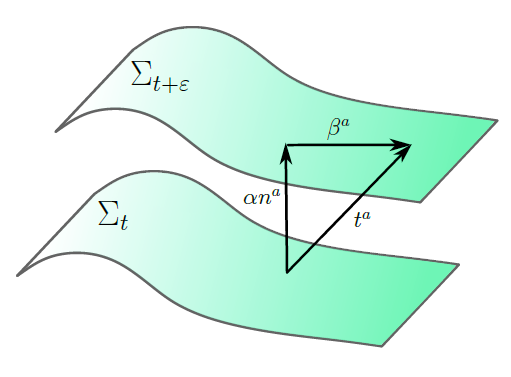
\includegraphics[width=\linewidth]{Screenshot 2025-11-22 121104.png}
    \caption{Slicing into spacelike hypersurfaces (Hilditch 2024)}
\end{figure}
\end{column}
\end{columns}
\vspace{5pt}
\begin{itemize}[<+->]
\item[]
\begin{block}{}
If we know these two quantities (as well as matter variables) at the initial hypersurface, we will be able to evolve it in time satisfying Einstein's equations even using regular computational methods
\end{block}
\end{itemize}
\end{frame}

\begin{frame}{Critical Phenomenon in Gravitational Collapse}
If we have some constraint satisfying initial data\footnote{Christodoulou
1990-2000} ($\gamma_{ab},K_{ab}$,Matter fields)
\begin{itemize}
    \item Sufficiently ``weak" Initial data :- Mass energy will get dispersed
    \item Sufficiently ``strong" Initial data :- Collapses to a singularity
\end{itemize}

Choptuik in his 1992 paper,
\begin{itemize}
    \item Took a spherically symmetric scalar field as matter source for $T_{ab}$
    \item He took several one-parameter families of initial data (by parameterizing the scalar field)
    \item In each family, he saw that at parameter p $>$ some ``Critical" parameter p*, it collapses (supercritical data) and p$<$p*  the scalar field disperses (subcritical data)
\end{itemize}
\end{frame}

\begin{frame}{Choptuik's findings}
But the groundbreaking thing he found was that, if we try to tune to this critical parameter p* and see the evolution, three remarkable features emerges 

\begin{enumerate}

\begin{columns}[T]

% ---------------- LEFT COLUMN ----------------
\begin{column}{0.55\linewidth}
\item Power-law mass scaling
\vspace{5pt}

The mass of the black hole that forms when $p > p^*$  
has no lower bound and follows the scaling law
\[
M_{\text{BH}} \propto (p - p^*)^{\gamma}.
\]
When $p < p^*$ ,the maximum of curvature invariants follow the scaling law
\[
I_{\text{max}} \propto (-p + p^*)^{-2\gamma}.
\]
\end{column}

% ---------------- RIGHT COLUMN ----------------
\hspace{-61pt}
\begin{column}{0.42\linewidth}
\begin{figure}
    \centering
    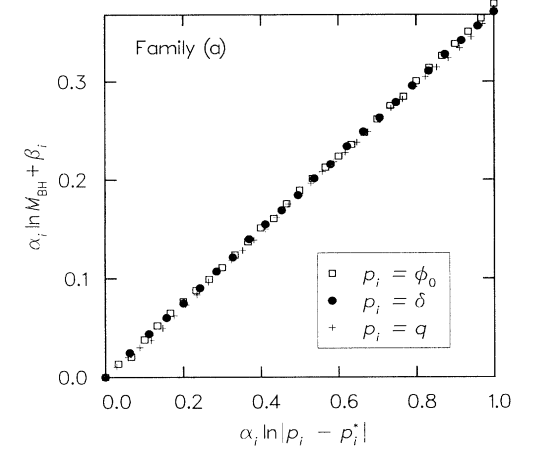
\includegraphics[width=1.4\linewidth]{image.png}
    \caption{Choptuik 1992}
\end{figure}
\end{column}
\end{columns}
\end{enumerate}
\end{frame}

\begin{frame}[noframenumbering]{Choptuik's findings}
But the groundbreaking thing he found was that, if we try to tune to this critical parameter p* and see the evolution, three remarkable features emerges 
\begin{enumerate}
    \begin{columns}[T]

% ---------------- LEFT COLUMN ----------------
\begin{column}{0.55\linewidth}

    
\setcounter{enumi}{1}
\item Universality of Critical exponent
\vspace{5pt}

The critical exponent $\gamma$ is universal across all families of initial data that share the same matter model and symmetry.
\end{column}

% ---------------- RIGHT COLUMN ----------------
\hspace{-61pt}
\begin{column}{0.42\linewidth}
\begin{figure}
    \centering
    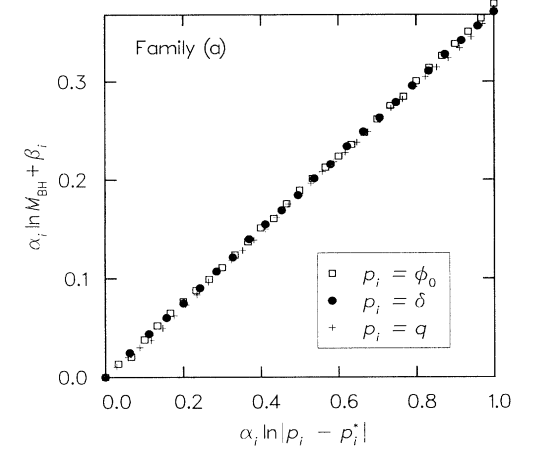
\includegraphics[width=1.3\linewidth]{image.png}
    \caption{Universality of critical exponent(Choptuik 1992)}
\end{figure}
\end{column}
\end{columns}
\end{enumerate}
\end{frame}
\begin{frame}[noframenumbering]{Choptuik's findings}
But the groundbreaking thing he found was that, if we try to tune to this critical parameter p* and see the evolution, three remarkable features emerges 
\begin{enumerate}
    \begin{columns}[T]

% ---------------- LEFT COLUMN ----------------
\hspace{40pt}
\begin{column}{0.80\linewidth}

    
\setcounter{enumi}{2}
\item Self similiarity and universality of Critical solution
\vspace{5pt}

 Critical solutions from all the families of initial data show self similarity in spatiotemporal scales

 \vspace{5pt}
 
$Z^*(a,b) \approx Z^*(a-\Delta,b-\Delta)$ where $\Delta$ is  called scale echoing constant (Same irrespective of initial data family)

\end{column}

% ---------------- RIGHT COLUMN ----------------

\begin{column}{0.42\linewidth}


\end{column}
\end{columns}
\end{enumerate}
\end{frame}

\section{Motivation}
\begin{frame}{Deviation from spherical symmetry}
\begin{itemize}
   
\item After this people did a lot of simulations with various matter models in spherical symmetry and was able to find similiar critical behaviour

\item As we deviate from spherical symmetry, we began to see a ``loss" in critical phenomenon. In the similiar massless scalar and vacuum field test done in axisymmetry, they found 
 
\end{itemize}
    
\vspace{-18pt}
\begin{figure}[h!]
\centering
\makebox[\textwidth][l]{%
    %\hspace*{-1.2cm}%  <-- SHIFT LEFT (adjust this)
    \begin{subfigure}{0.5\textwidth}
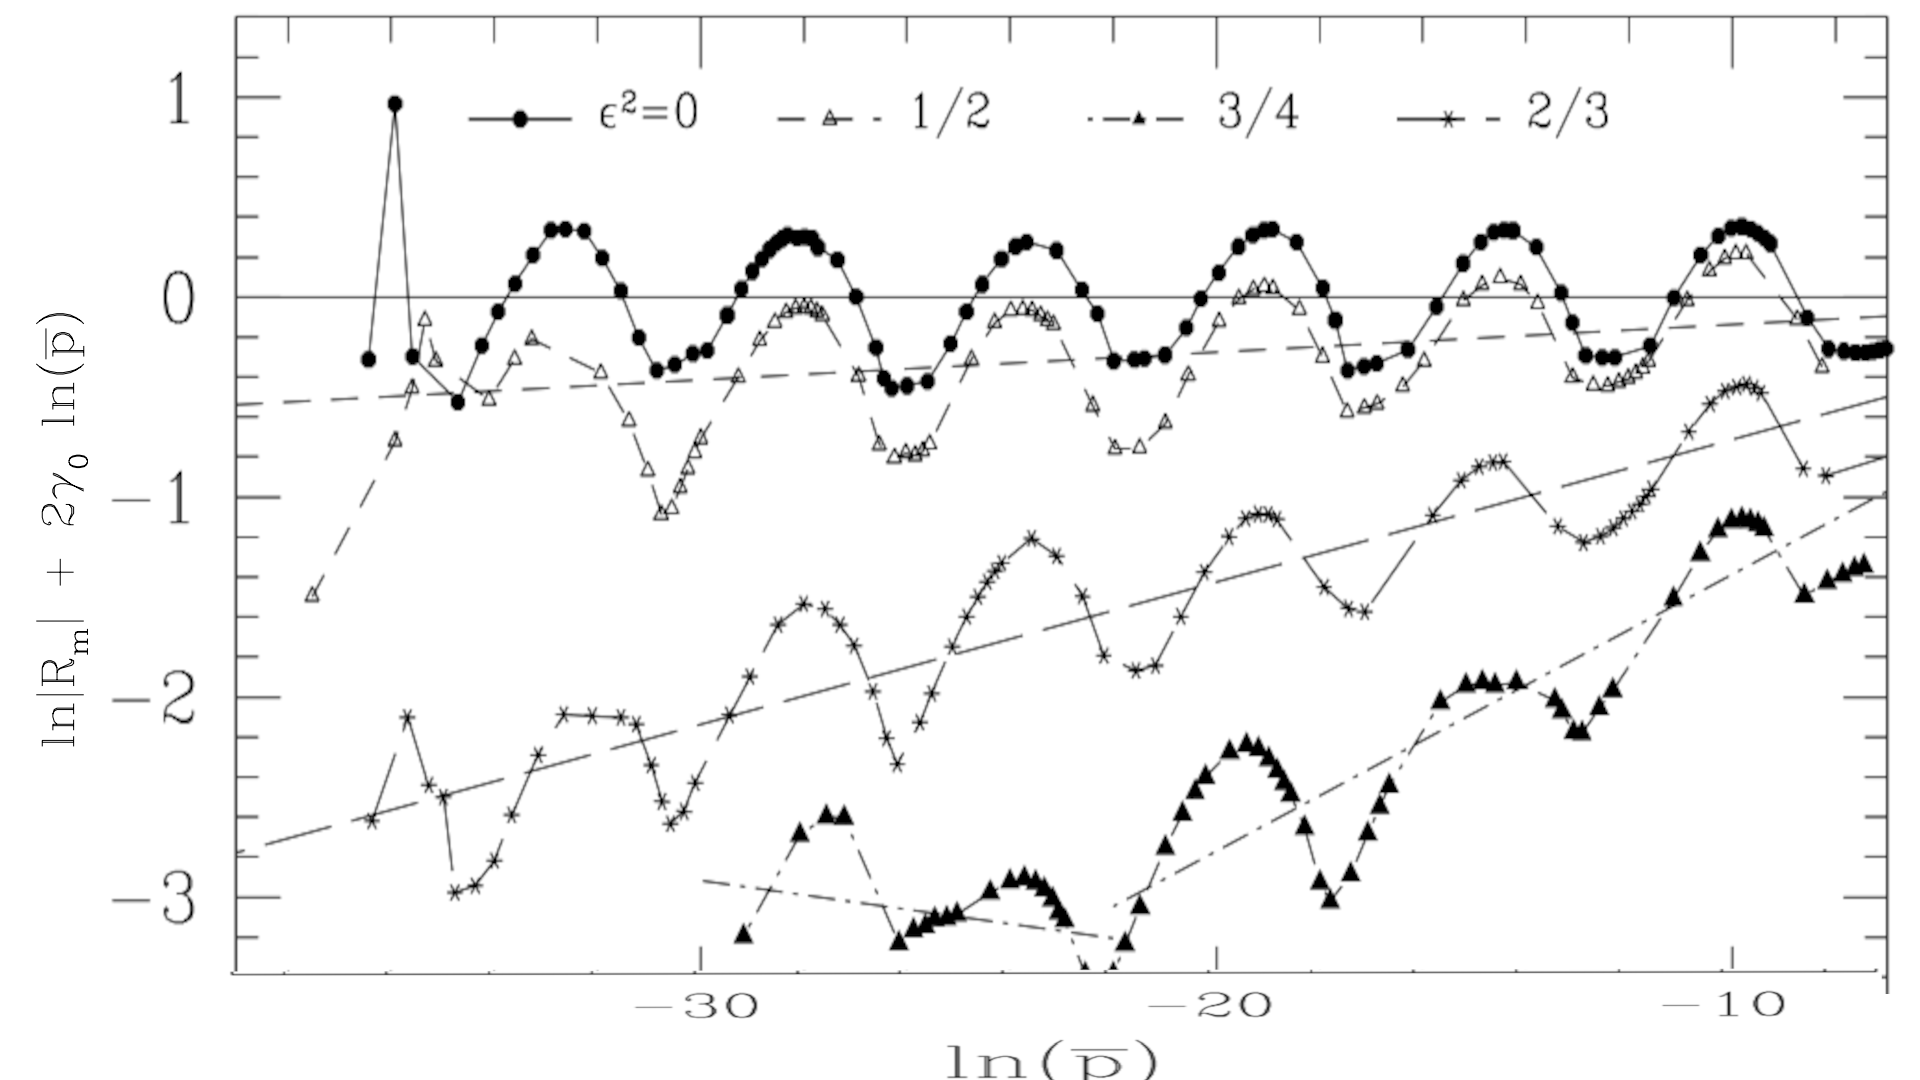
\includegraphics[width=1\linewidth]{fig.png}
        \caption{Matter without Angular momentum (Choptuik et al, 2003)}
    \end{subfigure}
    \hspace{0.5cm}
    \begin{subfigure}{0.45\textwidth}
        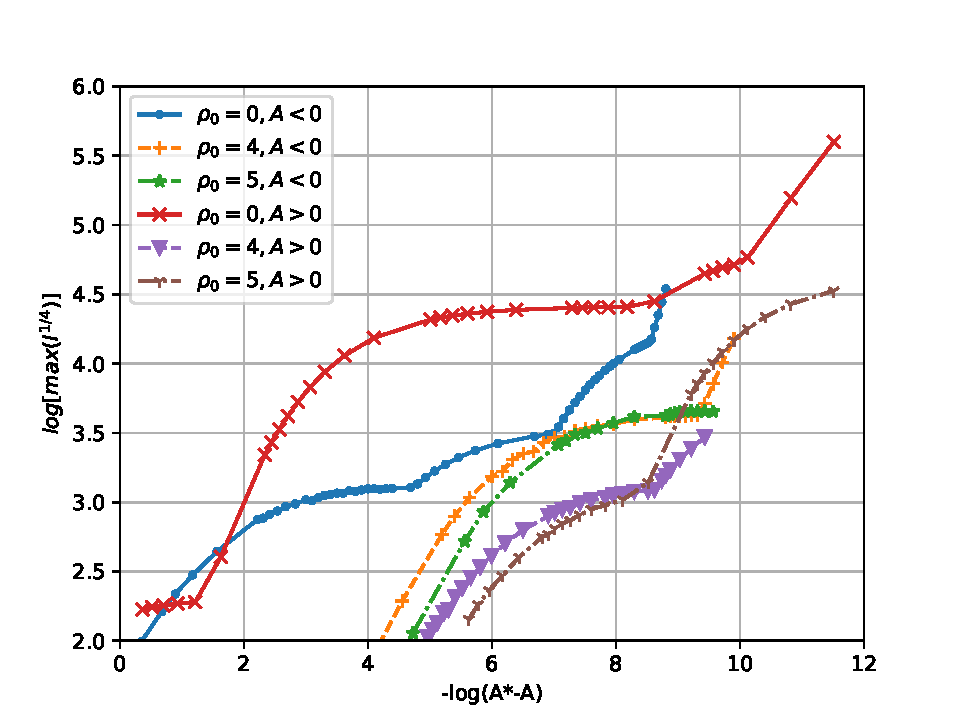
\includegraphics[width=1\linewidth]{Scaling_all.pdf}
        \caption{Twist free vacuum (Isabel Suarez Fernandez et al 2022)}
    \end{subfigure}
}
\end{figure}
\vspace{-10pt}
But on the introduction of \textbf{angular momentum} into the initial data in the case of scalar field, we begin to recover perfect critical phenomenon as before (Choptuik et al 2004)
\end{frame}
    




\begin{frame}{Motivation}
\vspace{-5pt}
\begin{columns}[T]
\begin{column}{0.50\linewidth}
But unlike in the case of matter, its not possible to generate angular momentum from regular initial data 

\end{column}  
\begin{column}{0.50\linewidth}
\begin{alertblock}{}
    \begin{itemize}
        \item Axisymmetry is characterised by the presence of a spacelike Killing vector field and twist measures its vorticity
         \item Angular Momentum $\implies$ Twist Twist $\centernot\implies$ Angular Momentum
    \end{itemize}
\end{alertblock}
\end{column}
\end{columns}

\begin{alertblock}{Motivation}
\begin{itemize}
    \item Until now all the vacuum tests that were done was in twist free conditions and it showed the same bad critical phenomenon as in angular momentum-free matter
    \item We are going to see how twist affects the critical phenomenon in this scenario and if it has some improvement angular momentum provides to matter
\end{itemize} 
\end{alertblock}
\end{frame}
\section{Progress}
\begin{frame}{Twisted Brill Initial Data construction}
\begin{itemize}

    \item Axisymmetric vacuum gravitational waves with $K_{ij}=0$ initial data is known as Brill waves. (This choice makes the momentum constraint be satisfied trivially)

    \item The usual twist excluded Brill wave ansatz 
\[
\gamma_{ij} = \psi^4 \tilde{\gamma}_{ij}(\rho,z)  = 
\psi ^4\begin{pmatrix}
    e^{2q(\rho,z)} & 0 & 0 \\
    0 & e^{2q(\rho,z)} & 0 \\
    0 & 0 & \rho^{2}
\end{pmatrix},
\]
when twist is zero, $\gamma_{i\phi} = 0$. Hence for including twist we add two more degrees of freedom at $\gamma_{i \phi}$

 \item We choose the twist included Brill wave ansatz 
    \[
\gamma_{ij} = \psi^4 \tilde{\gamma}_{ij}(\rho,z) =
\psi ^4\begin{pmatrix}
    e^{2q(\rho,z)} + f^2(\rho,z) & f(\rho,z)h(\rho,z) & \rho f(\rho,z) \\
    f(\rho,z)h(\rho,z) & e^{2q(\rho,z)} + h(\rho,z)^2 & \rho h(\rho,z) \\
    \rho f(\rho,z) & \rho h(\rho,z) & \rho^{2}
\end{pmatrix}
\]

\end{itemize}
\end{frame}
\begin{frame}{Twisted Brill Initial Data construction}
\begin{itemize}

\item Since the initial data have to be constraint satisfying we use Conformal-York decomposition method which converts the Hamiltonian contraint into an elliptic equation of the form
$$
8\tilde{D^2} \psi = \left(-\dfrac{e^{-2q}(\rho(\frac{\partial f}{\partial z} - {\frac{\partial h}{\partial \rho}}))+h)^2}{2 \rho^2}-2 \left(\dfrac{\partial^2 q}{\partial \rho^2}+ \dfrac{\partial^2 q}{\partial{z^2}}\right) \right) \psi
$$
  \item We choose the the following ansatz for the f and h 
    $$
    f(\rho,z) &= \texttt{tp1}\,\rho^{2} z\, e^{-(\rho^{2} + z^{2})} \; \; \;
h(\rho,z) &= \texttt{tp2}\,\rho^{3} e^{-(\rho^{2} + z^{2})}.
    $$

    \item As for the first family, we choose pure twisting (q=0) with \texttt{tp1}=\texttt{tp2} =p

 \item We solved the differential equation using the Psuedospectral method and the residuals are in the order of $10^{-30}$ and was checked for convergence with increasing resolution. \\
 \centering
 Hence, the \textbf{initial data} is ready to evolve now \greencheck

 We evolve that using the \texttt{bamps} NR framework
\end{itemize}
\end{frame}

\begin{frame}{Results}
\begin{itemize}
    \item Currently, we have tuned the critical parameter to about 3 decimal places for p positive and negative $p^* = 4.110 (\pm 0.003)$
\end{itemize}
\begin{figure}
    \centering
    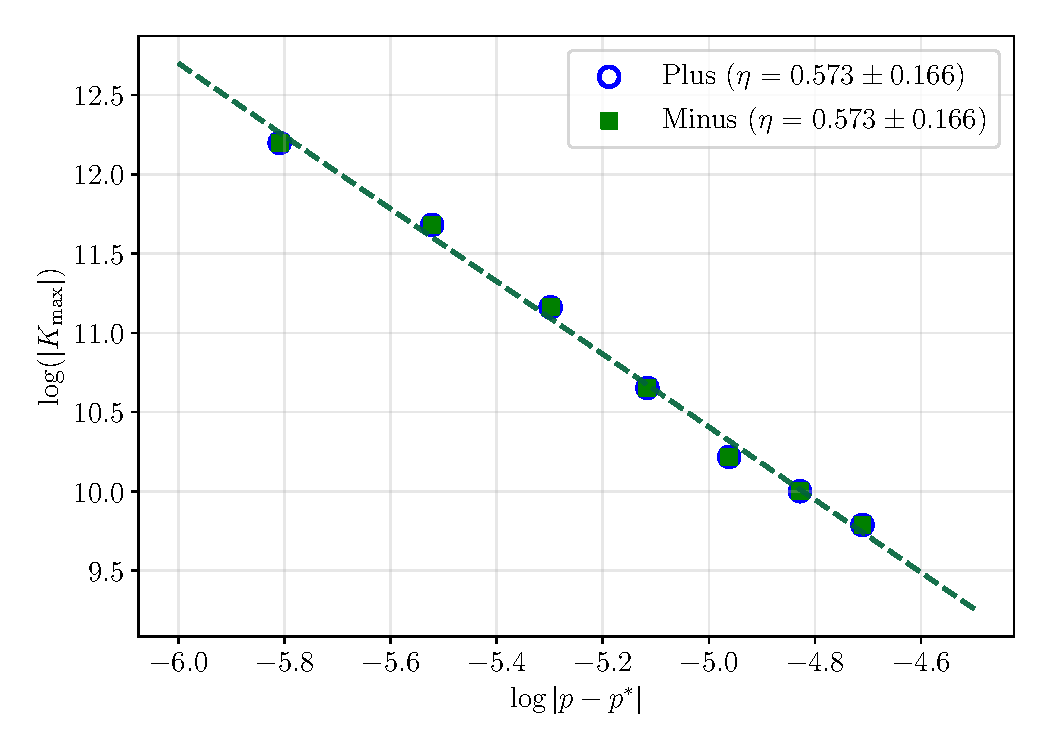
\includegraphics[width=0.6\linewidth]{../figures/separate_scaling_new.pdf}
\end{figure}
\begin{alertblock}{How do we tune?}
\begin{itemize}
    \item Eventhough we see the evidence of a power-law, we don't  currently report the critical exponent at face value since we haven't tuned enough
    \item It could be that we simply would not have reached the critical regime yet
\end{itemize} 
\end{alertblock}
\end{frame}
\begin{frame}{How do we tune and why is it hard?}

\vspace{150pt}
To observe subcriticality, we look at the dispersal of the Kretschmann Curvature scalar $K=R_{abcd}R^{abcd}$
    
\end{frame}
\begin{frame}{How do we tune and why is it hard?}
\vspace{150pt}
To observe supercriticality, we probe for the formation of \textbf{Apparent horizons} (AHs) in the slice. 

Singularity theorems guarantee a singular spacetime/formation of BH if AHs are formed in the spacetime.
\end{frame}


\begin{frame}{How do we tune and why is it hard?}
Often while tuning, we might not be able to classify the spacetimes due to some reasons which we hypothesised as

\begin{enumerate}
    \item Coordinate artifacts and gauge/slicing effects

    Solution:- In NR, they are mitigated by utilising the gauge freedom and changing the gauges to overcome the artifact. But this process requires trial and error, which slows down the tuning process.
\end{enumerate}
\vspace{100pt}
\end{frame}

\begin{frame}{How do we tune and why is it hard?}
    \noindent
    \hspace{-10pt}
    \begin{enumerate}[2]      
    \item \textbf{Limitations of Apparent Horizon finder}
    \begin{columns}[T]
\begin{column}{0.50\linewidth}
Apparent horizons are defined as outermost MOTS (Marginally Outer Trapped Surface) which are closed 2-surfaces that obeys the condition that the expansion of outgoing null geodesics emanating from it vanishes i.e  $$\Theta = D_i s^i + K_{ij} s^i s^j - K   = 0$$
where D is the induced 3-metric derivative, $K_{ij}$ the extrinsic curvature, $s^i$ the normal vector to the surface. We find surfaces that satisfies this condition.

\end{column}
\begin{column}{0.42\linewidth}
    \vspace{-30pt}
    \begin{figure}
        \centering
        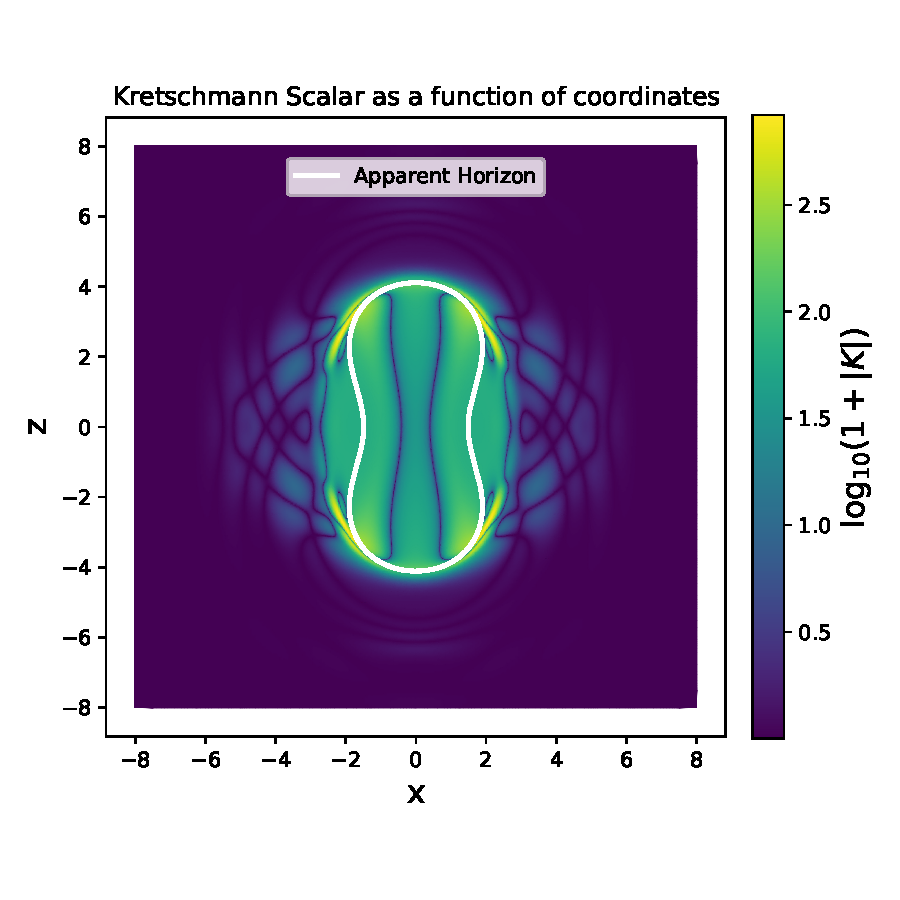
\includegraphics[width=1.2\linewidth]{figure.pdf}
        \caption{Apparent horizons that we usually find close to criticality in our experiments}
    \end{figure}
\end{column}

\end{columns}
    \end{enumerate}

\end{frame}

\begin{frame}{Horizon finding limitations}
\begin{columns}[T]
\begin{column}{0.60\linewidth}
\begin{itemize}
 \item We at first used the finder \texttt{AHLoc3D} which uses a spherical Strahlkorper / star-shaped parameterization where assume that the AH is star-shaped / a ray from a choosen center only touches the surface once. ($r=F(\theta)$ where r is the radius from a chosen center and $\theta$ the polar angle.)

 \item Since we were not able to go beyond 4.115 (towards 4.100), we rethought on this assumption and recently accounted for twist into a cartesian based AH finder which previously was made for non-twisting axisymmetry.


\end{itemize}
\end{column}
\begin{column}{0.42\linewidth}
\begin{figure}
    
    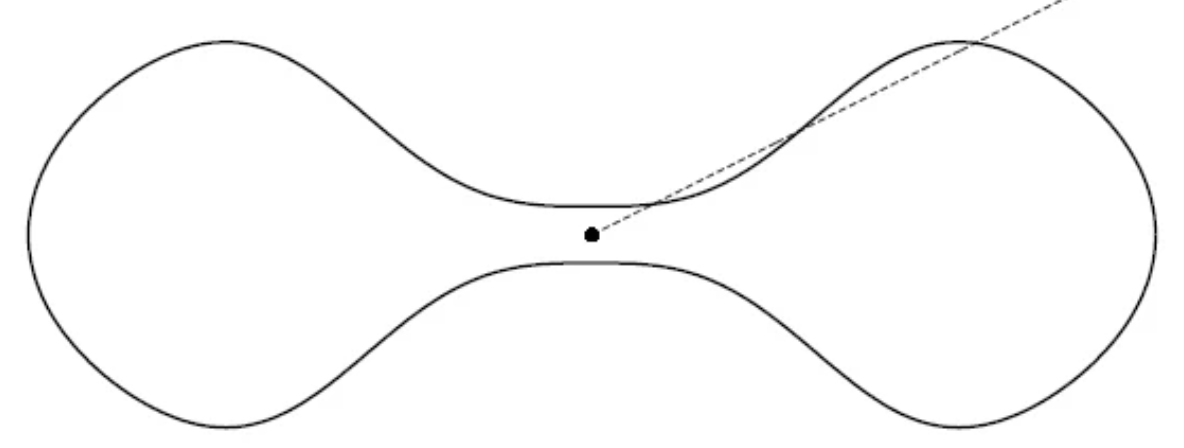
\includegraphics[scale=0.1]{../figures/Screenshot_2026-04-05_14-48-44.png}
    \caption{An example for a non-ray body horizon\footnotemark}
\end{figure}
\begin{alertblock}{Cartesian based finder}
    Previous studies in vacuum axisymmetry didn't necessitate the usage of a different parameterization since it very much simplifies the finding problem, and they were able to tune high values of precision.
\end{alertblock}
\footnotetext{Thornburg 2006}
\end{column}
\end{columns}  
\end{frame}

\begin{frame}{Horizon finding limitations}
    \vspace{-15pt}
   \begin{figure}
    \centering
    \hspace{-102pt}
    \begin{subfigure}{0.45\textwidth}
        \centering
        \includegraphics[width=0.9\linewidth]{../notebooks/figure_4.114.pdf}
        
    \end{subfigure}
    \hspace{-15pt}
    \begin{subfigure}{0.50\textwidth}
        \centering
        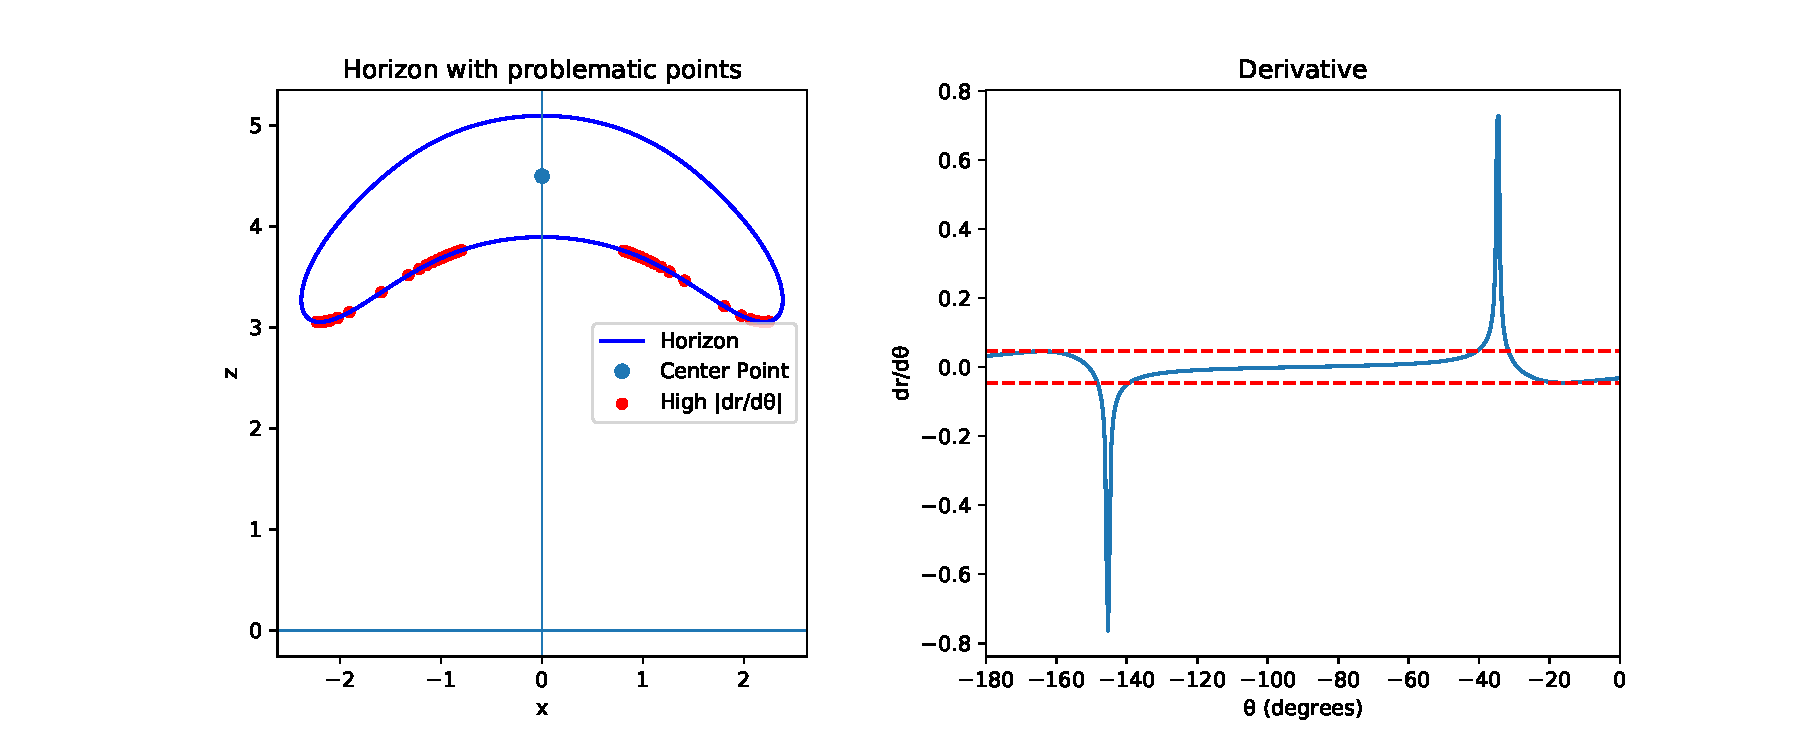
\includegraphics[width=1.7\linewidth]{../notebooks/problematic.pdf}
        \vspace{4pt}
    \end{subfigure}
\end{figure}
\vspace{-20pt}
\begin{itemize}
   \item We can see the limitation that \texttt{AHLoc3D} brings into the picture, the parameterization breaks at some points (shown in red) if we were to use the star shaped assumption
    \item The downside is that the new AH finder relies on ODE shooting method, which required substantial \textbf{manual intervention} unlike the automated \texttt{AHLoc3D} 
\end{itemize}
 \begin{alertblock}{}

\begin{itemize}
    \item Hence we expect that breakdown of the parameterisation was the real cause behind why we couldn't classify! \greencheck \textbf{We can continue tuning} \greencheck
\end{itemize}
\end{alertblock}  
\end{frame}

\begin{frame}{Conclusion and Future Directions}
    \textbf{Where We Stand:}
    \begin{itemize}
        \item Framework operational: twisting Brill waves with 3-decimal critical tuning even with significant computational cost per simulation (4000 core hours/simulations)
        \item New modified Cartesian AH finder dramatically improves the tuning procedure towards the critical threshold 
    \end{itemize}
    
    \vspace{0.3cm}
    \textbf{Critical Questions to Answer:}
    \begin{itemize}
        \item What are the critical exponents and other constants for twisting vacuum?
        \item Is the phenomenon universal across different families?
        \item Does twist fundamentally alter the critical solution structure?
    \end{itemize}
    
    \vspace{0.3cm}
    \textbf{Strategy:} Higher precision tuning → Multiple families → Teukolsky waves → Universality test
\end{frame}
\begin{frame}{Acknowledgement}
    \begin{itemize}
        \item My sincere gratitude to my guide, Dr. Soumen Basak, for his continuous guidance and support.
    \item Thank you to Dr.David Hilditch (CENTRA, Lisbon), Dr.Ananya Adhikari(CENTRA, Lisbon), Dr.Prayush Kumar (ICTS,Bangalore) for their helpful discussion regarding Numerical Relativity, setting up the code base and computational time 
    \item Heartfelt appreciation to my family and my friends for their encouragement throughout this work.
    \end{itemize}
\end{frame}
\appendix
\section*{Backup}
\setbeamertemplate{footline}{}
\setbeamertemplate{headline}{}
\setbeamertemplate{navigation symbols}{}
\begin{frame}{Deviation from spherical symmetry}
\begin{columns}
\begin{column}{0.52\linewidth}
\begin{itemize}

    \vspace{-10pt}
    \item Hence a perfect notion of universal critical exponent and echoing period is lost which now varies with family
    \item Center of collapse bifurcates into two
    \item Complicated notion of self similarity of critical solution
\end{itemize}
\end{column}
\begin{column}{0.42\linewidth}
    \begin{figure}
        \centering
        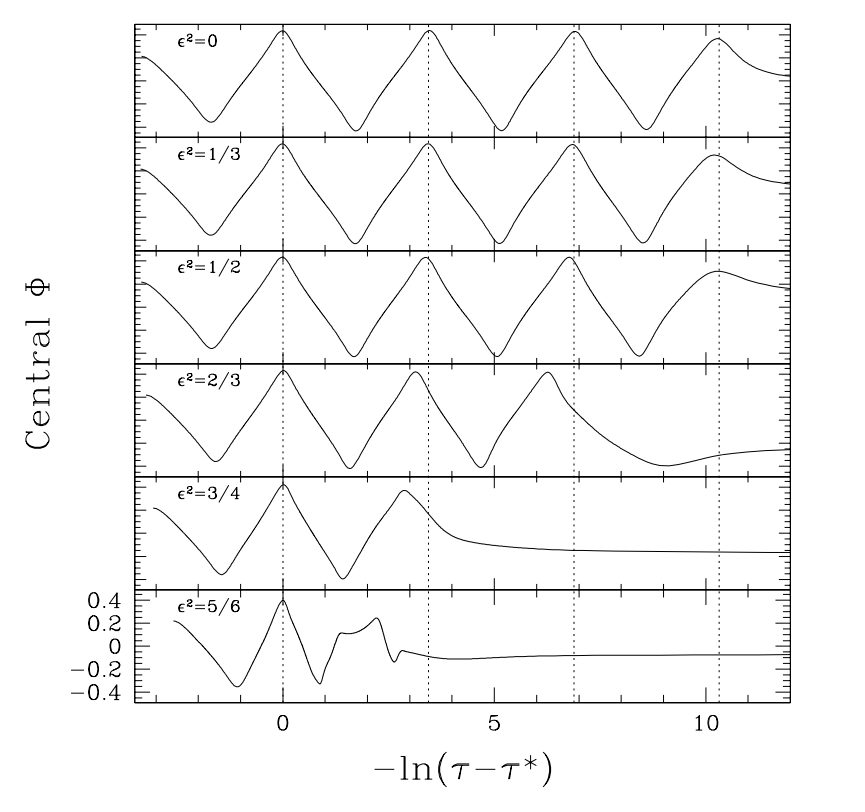
\includegraphics[width=1\linewidth]{echoing_loss.png}
        \caption{Complicated self similarity(Choptuik et al, 2003)}
        \label{fig:placeholder}
    \end{figure}
\end{column}
\end{columns}
\end{frame}
\begin{frame}{Twist and angular momentum}
\begin{itemize}
    \item Axisymmetry is defined by the existence of a killing vector field $\xi^a =(\partial_\phi)^a$ and twist ($\omega_a$) measures its failure to be hypersurface orthogonal.
    \item From the idea of Komar angular momentum and its conservation, J = $ J_{BH} +J_{Matter}$ ie Black holes formed from vacuum axisymmetric collapse are non rotating (no angular momentum)
    \begin{alertblock}{}  
\item But when twist is 0, there won't be angular momentum as well
$$
J=\dfrac{1}{32\pi^2\lambda} \oint_{\partial S_t} \epsilon_{abcd} \xi^c \omega^d dS^{ab} 
$$
Hence in vacuum there can be twist even without angular momentum (since $J_{BH}$ and $J_{Matter}$  vanishes)


\end{alertblock}
\end{itemize}
\end{frame}
\begin{frame}{Construction of one-parameter families of initial data}

\begin{itemize}
  
    
    \item A general axisymmetric, regular metric can be written as: (Rinne 2006)

\[
\gamma_{ij} =
\begin{bmatrix}
H + \rho ^2 J & \rho E & \rho ^3 K \\
\rho E & C & \rho ^2 G \\
\rho ^3 K & \rho ^2 G & \rho ^2 (H - \rho ^2 J)
\end{bmatrix}
\]

Here the functions \(H, E, C, G, K, J\) are even in \(\rho \) 
(i.e.\ they depend on \(\rho ^2\)) and depend on \(z\).
\end{itemize}

    
\end{frame}
\begin{frame}{Choptuik's findings}
But the groundbreaking thing he found was that, if we try to tune to this critical parameter p* and see the evolution, three remarkable features emerges 
When $p < p^*$ ,the maximum of curvature invariants follow the scaling law
\[
I_{\text{max}} \propto (-p + p^*)^{-2\gamma}.
\]
\begin{enumerate}

\begin{columns}[T]

% ---------------- LEFT COLUMN ----------------
\begin{column}{0.55\linewidth}
\item Power-law mass scaling
\vspace{5pt}

When $p < p^*$ ,the maximum of curvature invariants follow the scaling law
\[
I_{\text{max}} \propto (-p + p^*)^{-2\gamma}.
\]

\end{column}

% ---------------- RIGHT COLUMN ----------------
\hspace{-61pt}
\begin{column}{0.42\linewidth}

\begin{figure}
    \centering
    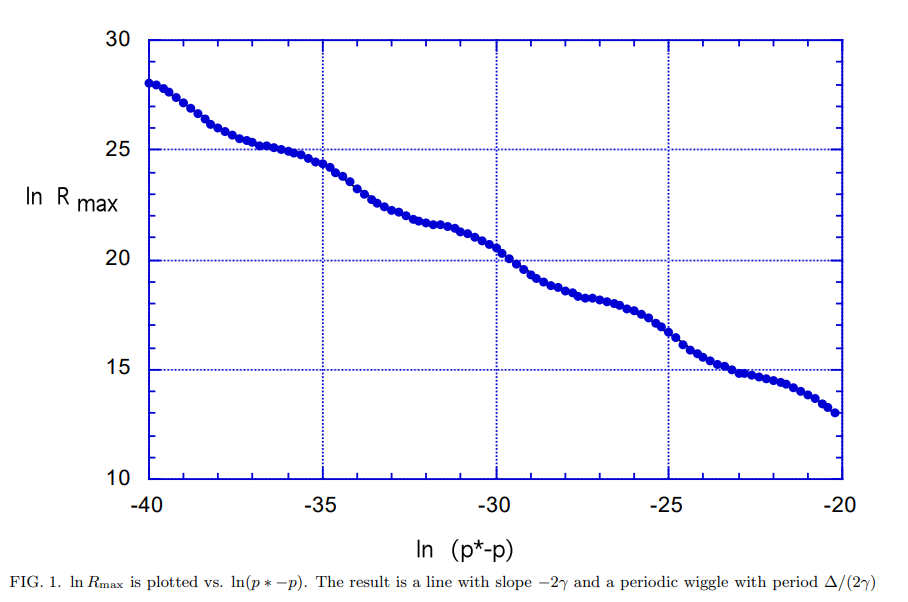
\includegraphics[width=1.4\linewidth]{scaling_curvature.png}
    \caption{Scaling of curvature scalar (maximum)}
    \label{fig:placeholder}
\end{figure}
\end{column}
\end{columns}
\end{enumerate}
\end{frame}

\begin{frame}{Construction}
\begin{itemize}
  

 \item Additionally to check whether the constraints are satisified (If we have solved the correct differential equation) we use the \texttt{bamps} framework which we use for time evolutions of our initial data
    \begin{figure}
\makebox[\textwidth][l]{%
    \hspace*{-40pt}%  <-- SHIFT LEFT (adjust this)
    \begin{subfigure}{0.50\textwidth}
        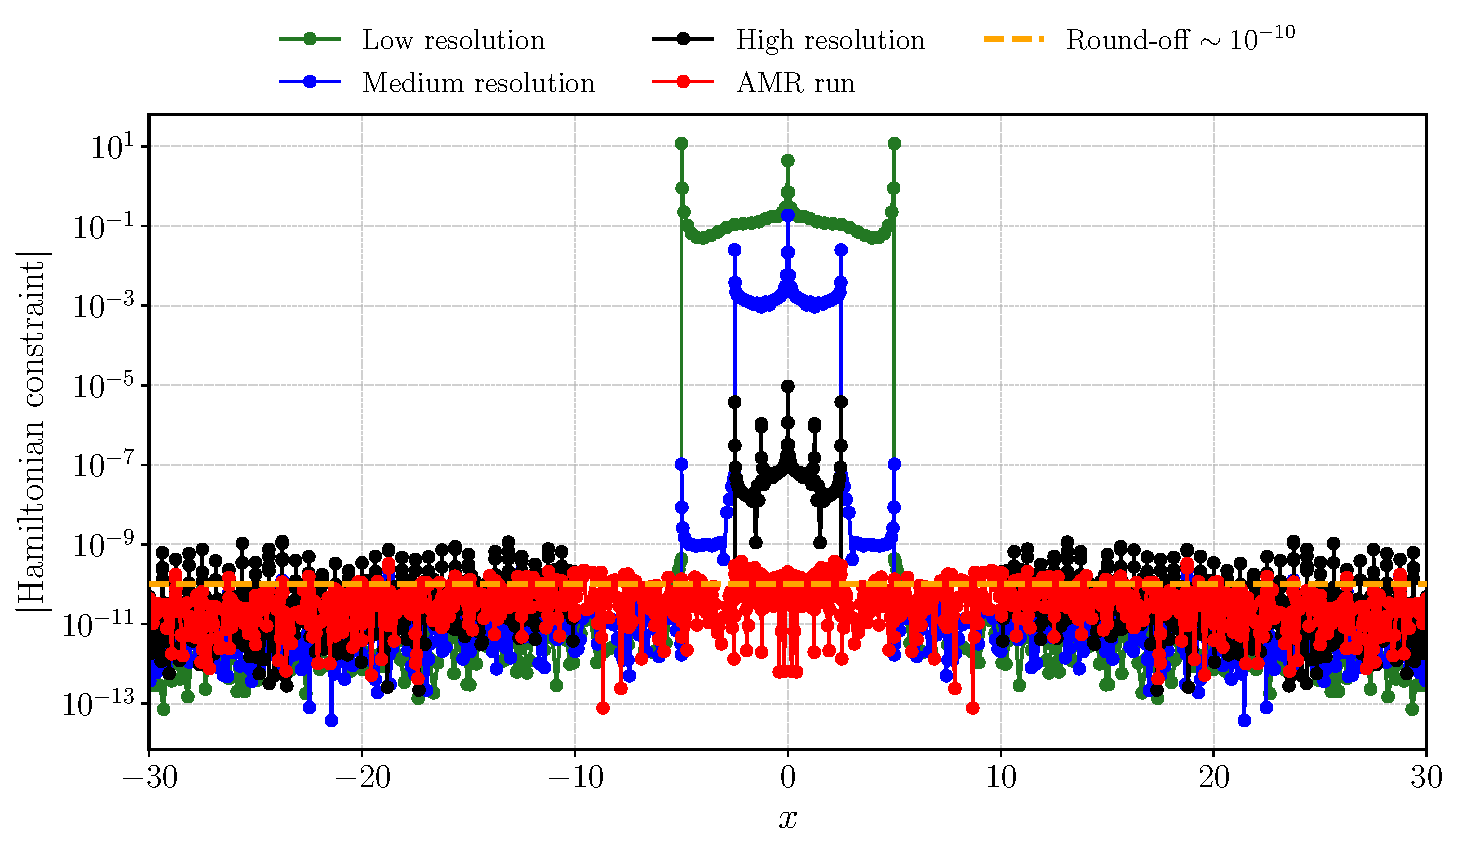
\includegraphics[width=1.1\linewidth]{plots/constraint_plot_reflected_x.pdf}
        \caption{$x$ direction}
    \end{subfigure}
    \hspace{0.5cm}
    \begin{subfigure}{0.5\textwidth}
        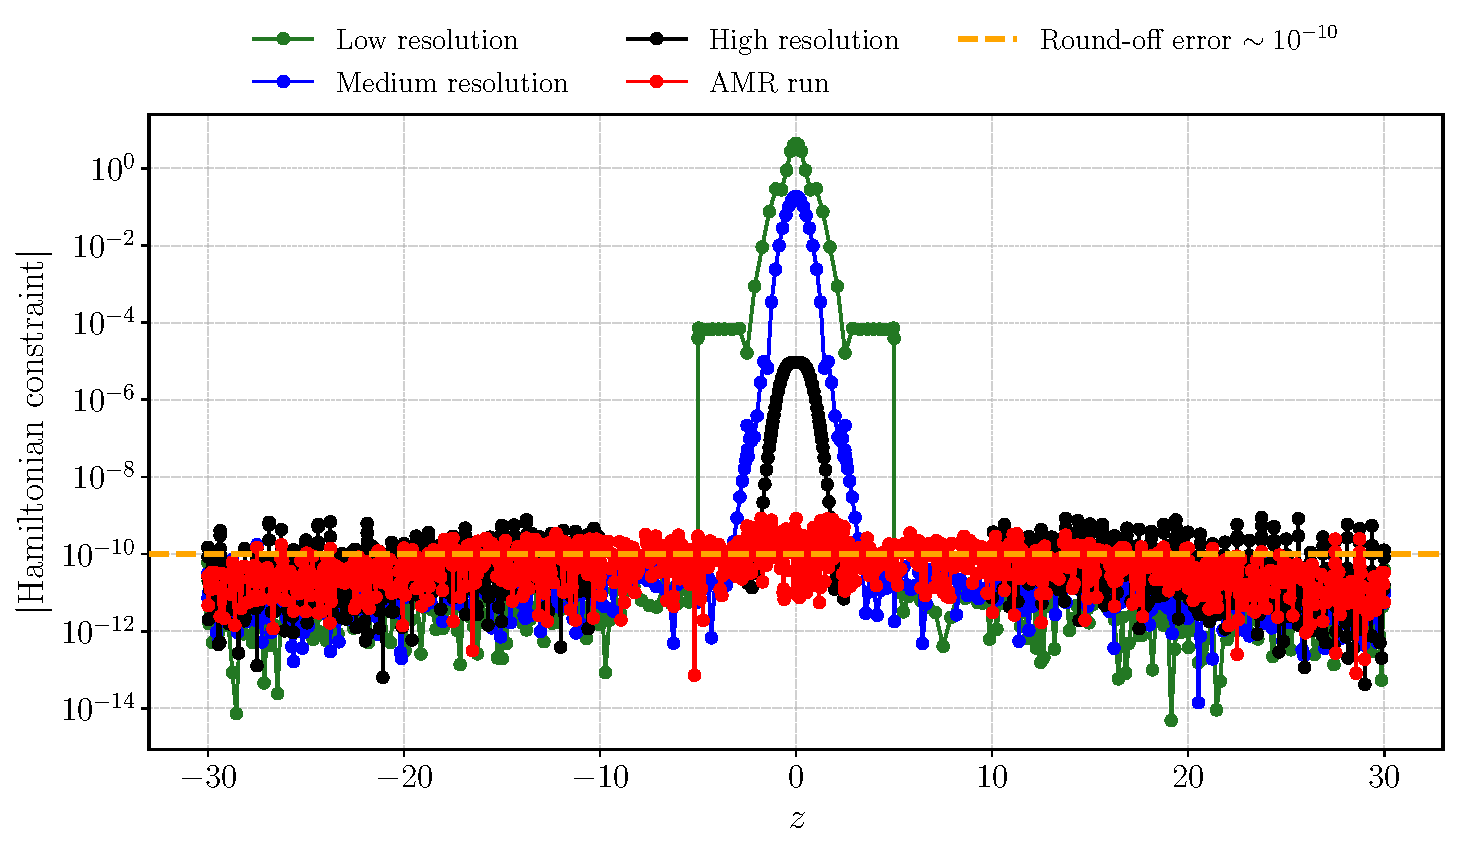
\includegraphics[width=1.1\linewidth]{plots/constraint_plot_z.pdf}
        \caption{$z$ direction}
    \end{subfigure}
}
Hence the initial data is ready to evolve now \greencheck
\end{figure}
\end{itemize}
\end{frame}
\begin{frame}{~}
    
\end{frame}

\begin{frame}{GR into a time evolution problem}

\vspace{5pt}
Often in time evolution PDE problems, the relevent equations can be formulated of the form.
$$
\partial_t u = f(u, \partial_{x^i} u)
$$
where t is the time and $x^i$ is the spatial coordinates (+ some contraint equations)
$$
R_{\mu \nu}-\frac{1}{2}g_{\mu \nu}R =8 \pi T_{\mu \nu}
$$
\textbf{BUT}, One of the most important equation of GR, the Einstein's Field equations, which are system of non-linear coupled differential equations, does'nt have that form explicitly
\end{frame}

\begin{frame}{Introduction of angular momentum}

\begin{columns}
    \begin{column}{0.52\linewidth}
        \begin{figure}
            \centering
            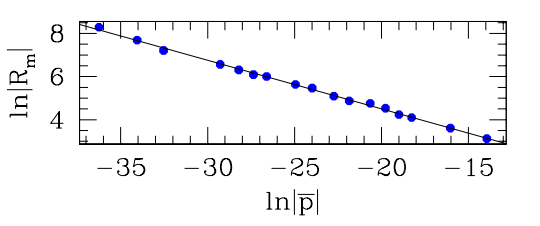
\includegraphics[width=0.95\linewidth]{chop_getcrit.png}
            \caption{Choptuik massless scalar field with angular momentum (Choptuik et al 2004)}
            \label{fig:placeholder}
        \end{figure}
 $\Delta = 0.42 \pm 4\%, \qquad \gamma = 0.11 \pm 10\%$
        \end{column}
        \begin{column}{0.41\linewidth}
        \begin{block}{}
            \begin{itemize}
                \item But what about vacuum ?
                \item Earlier spherical symmetry prevents pure gravitational wave and its collapse but axisymmetry does not !\footnote{Christodoulou
1990-2000}
            \end{itemize}
            \end{block}
    \end{column}
\end{columns}
\end{frame}

\begin{frame}{Vacuum and angular momentum}
\begin{columns}
 \hspace{-10pt}
    \begin{column}{0.65\linewidth}
    \begin{figure}
        \centering
        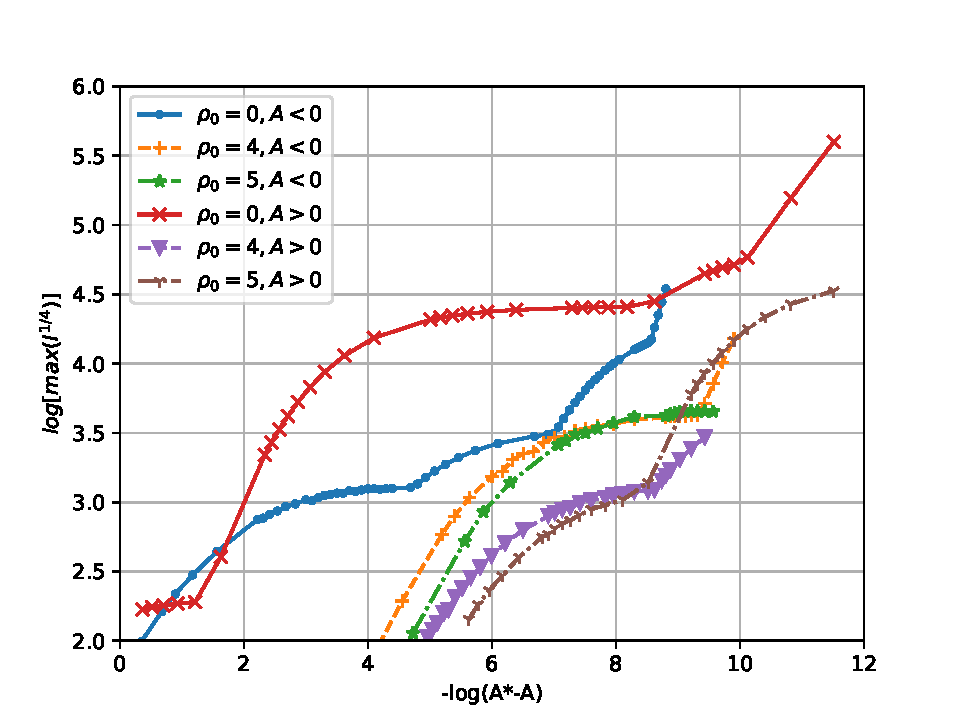
\includegraphics[width=1\linewidth]{Scaling_all.pdf}
        \caption{No proper critical phenomenon (Isabel Suarez Fernandez et al 2022)}
        \label{fig:placeholder}
    \end{figure}
\end{column}
\hspace{-10pt}
\begin{column}{0.50\linewidth}
\vspace{-30pt} 
\begin{block}{}
\begin{itemize}
    \item Even in axisymmetric vacuum gravitational wave collapse, we see the same
    \item But unlike in the case of matter, its not possible to generate angular momentum from regular initial data 
\end{itemize}
\end{block}
\begin{alertblock}{}
    \begin{itemize}
        \item Axisymmetry is characterised by the presence of a spacelike Killing vector field and twist measures its vorticity
         \item Angular Momentum $\implies$ Twist Twist $\centernot\implies$ Angular Momentum
    \end{itemize}
\end{alertblock}
\end{column}
\end{columns}
\end{frame}

\end{document}
